\documentclass[12pt]{ociamthesis}
\usepackage{amssymb}

\title{Template Laporan Tingkat Akhir\\[1ex]
        Internship II atau Tugas Akhir}

\author{Nama Mahasiswa}
\college{NPM\\[5ex]
In Partial Fulfilment of The Requirements for
The Degree of Applied Bachelor of Informatics Engineering}

\degree{Politeknik Pos Indonesia}
\degreedate{Bandung 2018}

\begin{document}

\baselineskip=18pt plus1pt

\setcounter{secnumdepth}{3}
\setcounter{tocdepth}{3}


\maketitle                  
\begin{dedication}
`Jika Kamu tidak dapat menahan lelahnya belajar, \\
Maka kamu harus sanggup menahan perihnya Kebodohan.'\\ 
~Imam Syafi'i~\\
\end{dedication}        
\begin{acknowledgements}
Pertama-tama kami panjatkan puji dan syukur kepada Allah SWT yang telah memberikan rahmat dan hidayah-Nya sehingga Buku Pedoman Tingkat Akhir ini dapat diselesaikan.
\end{acknowledgements}   
\begin{abstract}
	Buku Pedoman ini dibuat dengan tujuan memberikan acuan, bagi mahasiswa Tingkat Akhir dan dosen
	Pembimbing. Pada intinya buku ini menjelaskan secara lengkap tentang Standar pengerjaan Intership  dan 
	Tugas Akhir
	di Program Studi D4 Teknik Informatika, dan juga mengatur mekanisme, teknik penulisan, serta
	penilaiannya.Dengan demikian diharapkan semua pihak yang terlibat dalam aktivitas Bimbingan Mahasiswa Tingkat Akhir
	berjalan lancar dan sesuai dengan standar.
\end{abstract}          

\begin{romanpages}
\tableofcontents
\listoffigures
\end{romanpages}

\begin{center}
  \textbf{Rekomendasi Penilaian}
\end{center}
Untuk memenuhi kelulusan Internship II \textbf{Syarat Kelulusan} :
\begin{enumerate}
  \item Dedikasi
  \item Produktifitas
  \item Integritas
  \item Disiplin
  \item Loyalitas
\end{enumerate}
Adapun \textbf{Syarat Khusus} :
\begin{enumerate}
  \item Kreatif Inisiatif
\end{enumerate}

\textbf{Keterangan}
\begin{enumerate}
\item Dedikasi
Berikut kategori penilaian dediskasi pada Tabel \ref{table:Dedikasi}
\begin{table}[!htbp]
\centering
\begin{tabular}{ |c|c|c|c|c|c|c|c|c|c| }
\hline
No. & Label & Nilai & Keterangan \\
\hline
1 & \textbf{TINGGI} & 3 & Full commit selama 5 hari kerja pada repositori buku informatika \\
\hline
2 & \textbf{SEDANG} & 2 & 4 hari kerja \\
\hline
3 & \textbf{RENDAH} & 1 & 0 s/d 3 hari kerja \\
\hline
\end{tabular}
\caption{Tabel Dedikasi}
\label{table:Dedikasi}
\end{table}

\item Produktifitas
Berikut kategori penilaian Profuktifitas pada Tabel \ref{table:Produktifitas}
\begin{table}[!htbp]
\centering
\begin{tabular}{ |c|c|c|c|c|c|c|c|c|c| }
\hline
No. & Label & Nilai & Keterangan \\
\hline
1 & \textbf{TINGGI} & 3 & Mengerjakan 5 pekerjaan harian \\
\hline
2 & \textbf{SEDANG} & 2 & Mengerjakan 4 pekerjaan harian \\
\hline
3 & \textbf{RENDAH} & 1 & Mengerjakan 0 s/d 3 pekerjaan harian \\
\hline
\end{tabular}
\caption{Tabel Produktifitas}
\label{table:Produktifitas}
\end{table}  

\item Integritas
Berikut kategori penilaian Integritas pada Tabel \ref{table:Integritas}
\begin{table}[!htbp]
\centering
\begin{tabular}{ |c|c|c|c|c|c|c|c|c|c| }
\hline
No. & Label & Nilai & Keterangan \\
\hline
1 & \textbf{TINGGI} & 3 & Tidak ada penolakan pull request selama 5 hari kerja \\
\hline
2 & \textbf{SEDANG} & 2 & Ada 1 penolakan dalam 1 minggu \\
\hline
3 & \textbf{RENDAH} & 1 & Lebih dari satu penolakan dalam 1 minggu \\
\hline
\end{tabular}
\caption{Tabel Integritas}
\label{table:Integritas}
\end{table}  

\item Disiplin
Berikut kategori penilaian Disiplin pada Tabel \ref{table:Disiplin}
\begin{table}[!htbp]
\centering
\begin{tabular}{ |c|c|c|c|c|c|c|c|c|c| }
\hline
No. & Label & Nilai & Keterangan \\
\hline
1 & \textbf{TINGGI} & 3 & Dalam satu minggu datang sebelum jam 9 pulang setelah jam 15 \\
\hline
2 & \textbf{SEDANG} & 2 & Ada satu hari telat \\
\hline
3 & \textbf{RENDAH} & 1 & Lebih dari satu hari telat \\
\hline
\end{tabular}
\caption{Tabel Disiplin}
\label{table:Disiplin}
\end{table}  

\item Loyalitas
Berikut kategori penilaian Loyalitas pada Tabel \ref{table:Loyalitas}
\begin{table}[!htbp]
\centering
\begin{tabular}{ |c|c|c|c|c|c|c|c|c|c| }
\hline
No. & Label & Nilai & Keterangan \\
\hline
1 & \textbf{TINGGI} & 3 & Selama satu minggu Area kerja bersih tanpa ada debu dan indah, perangkat ada yang dijaga atau diperbaiki \\
\hline
2 & \textbf{SEDANG} & 2 & Ada satu hari area kerja tidak bersih dari debu dan berantakan, dan atau perangkat ada yang rusak \\
\hline
3 & \textbf{RENDAH} & 1 & Lebih dari satu hari, area kerja berantakan dan tidak ada perangkat yang jalan atau diperbaiki \\
\hline
\end{tabular}
\caption{Tabel Loyalitas}
\label{table:Loyalitas}
\end{table}  

\item Kreatif dan Inisiatif
Berikut kategori penilaian Kreatif dan Inisiatif pada Tabel \ref{table:KnI}
\begin{table}[!htbp]
\centering
\begin{tabular}{ |c|c|c|c|c|c|c|c|c|c| }
\hline
No. & Label & Nilai & Keterangan \\
\hline
1 & \textbf{TINGGI} & 3 & Menjadi tentor dengan jumlah peserta minimal 10 orang berbayar atau bersponsor \\
\hline
2 & \textbf{SEDANG} & 2 & Menjadi tentor dengan jumlh peserta minimal 5 orang berbayar atau bersponsor \\
\hline
3 & \textbf{RENDAH} & 1 & Selain kategori diatas \\
\hline
\end{tabular}
\caption{Tabel Kreatif dan Inisiatif}
\label{table:KnI}
\end{table} 
\end{enumerate}
\textbf {Ketentuan}
\begin{enumerate}
  \item Nilai minimal syarat umum adalah 13 dari rata2 minimall 20 minggu. apabila kurang dari 13 maka bisa menambah lagi waktu intership sesuai dengan kebutuhan nilai minimum.
  \item Syarat khusus bisa diselenggarakan minimal sekali dengan minimal nilai sedang
\end{enumerate} 

\chapter{Iqbal Syarif Awalludin (1144095)}
\begin{figure}[!htbp]
  \centering
  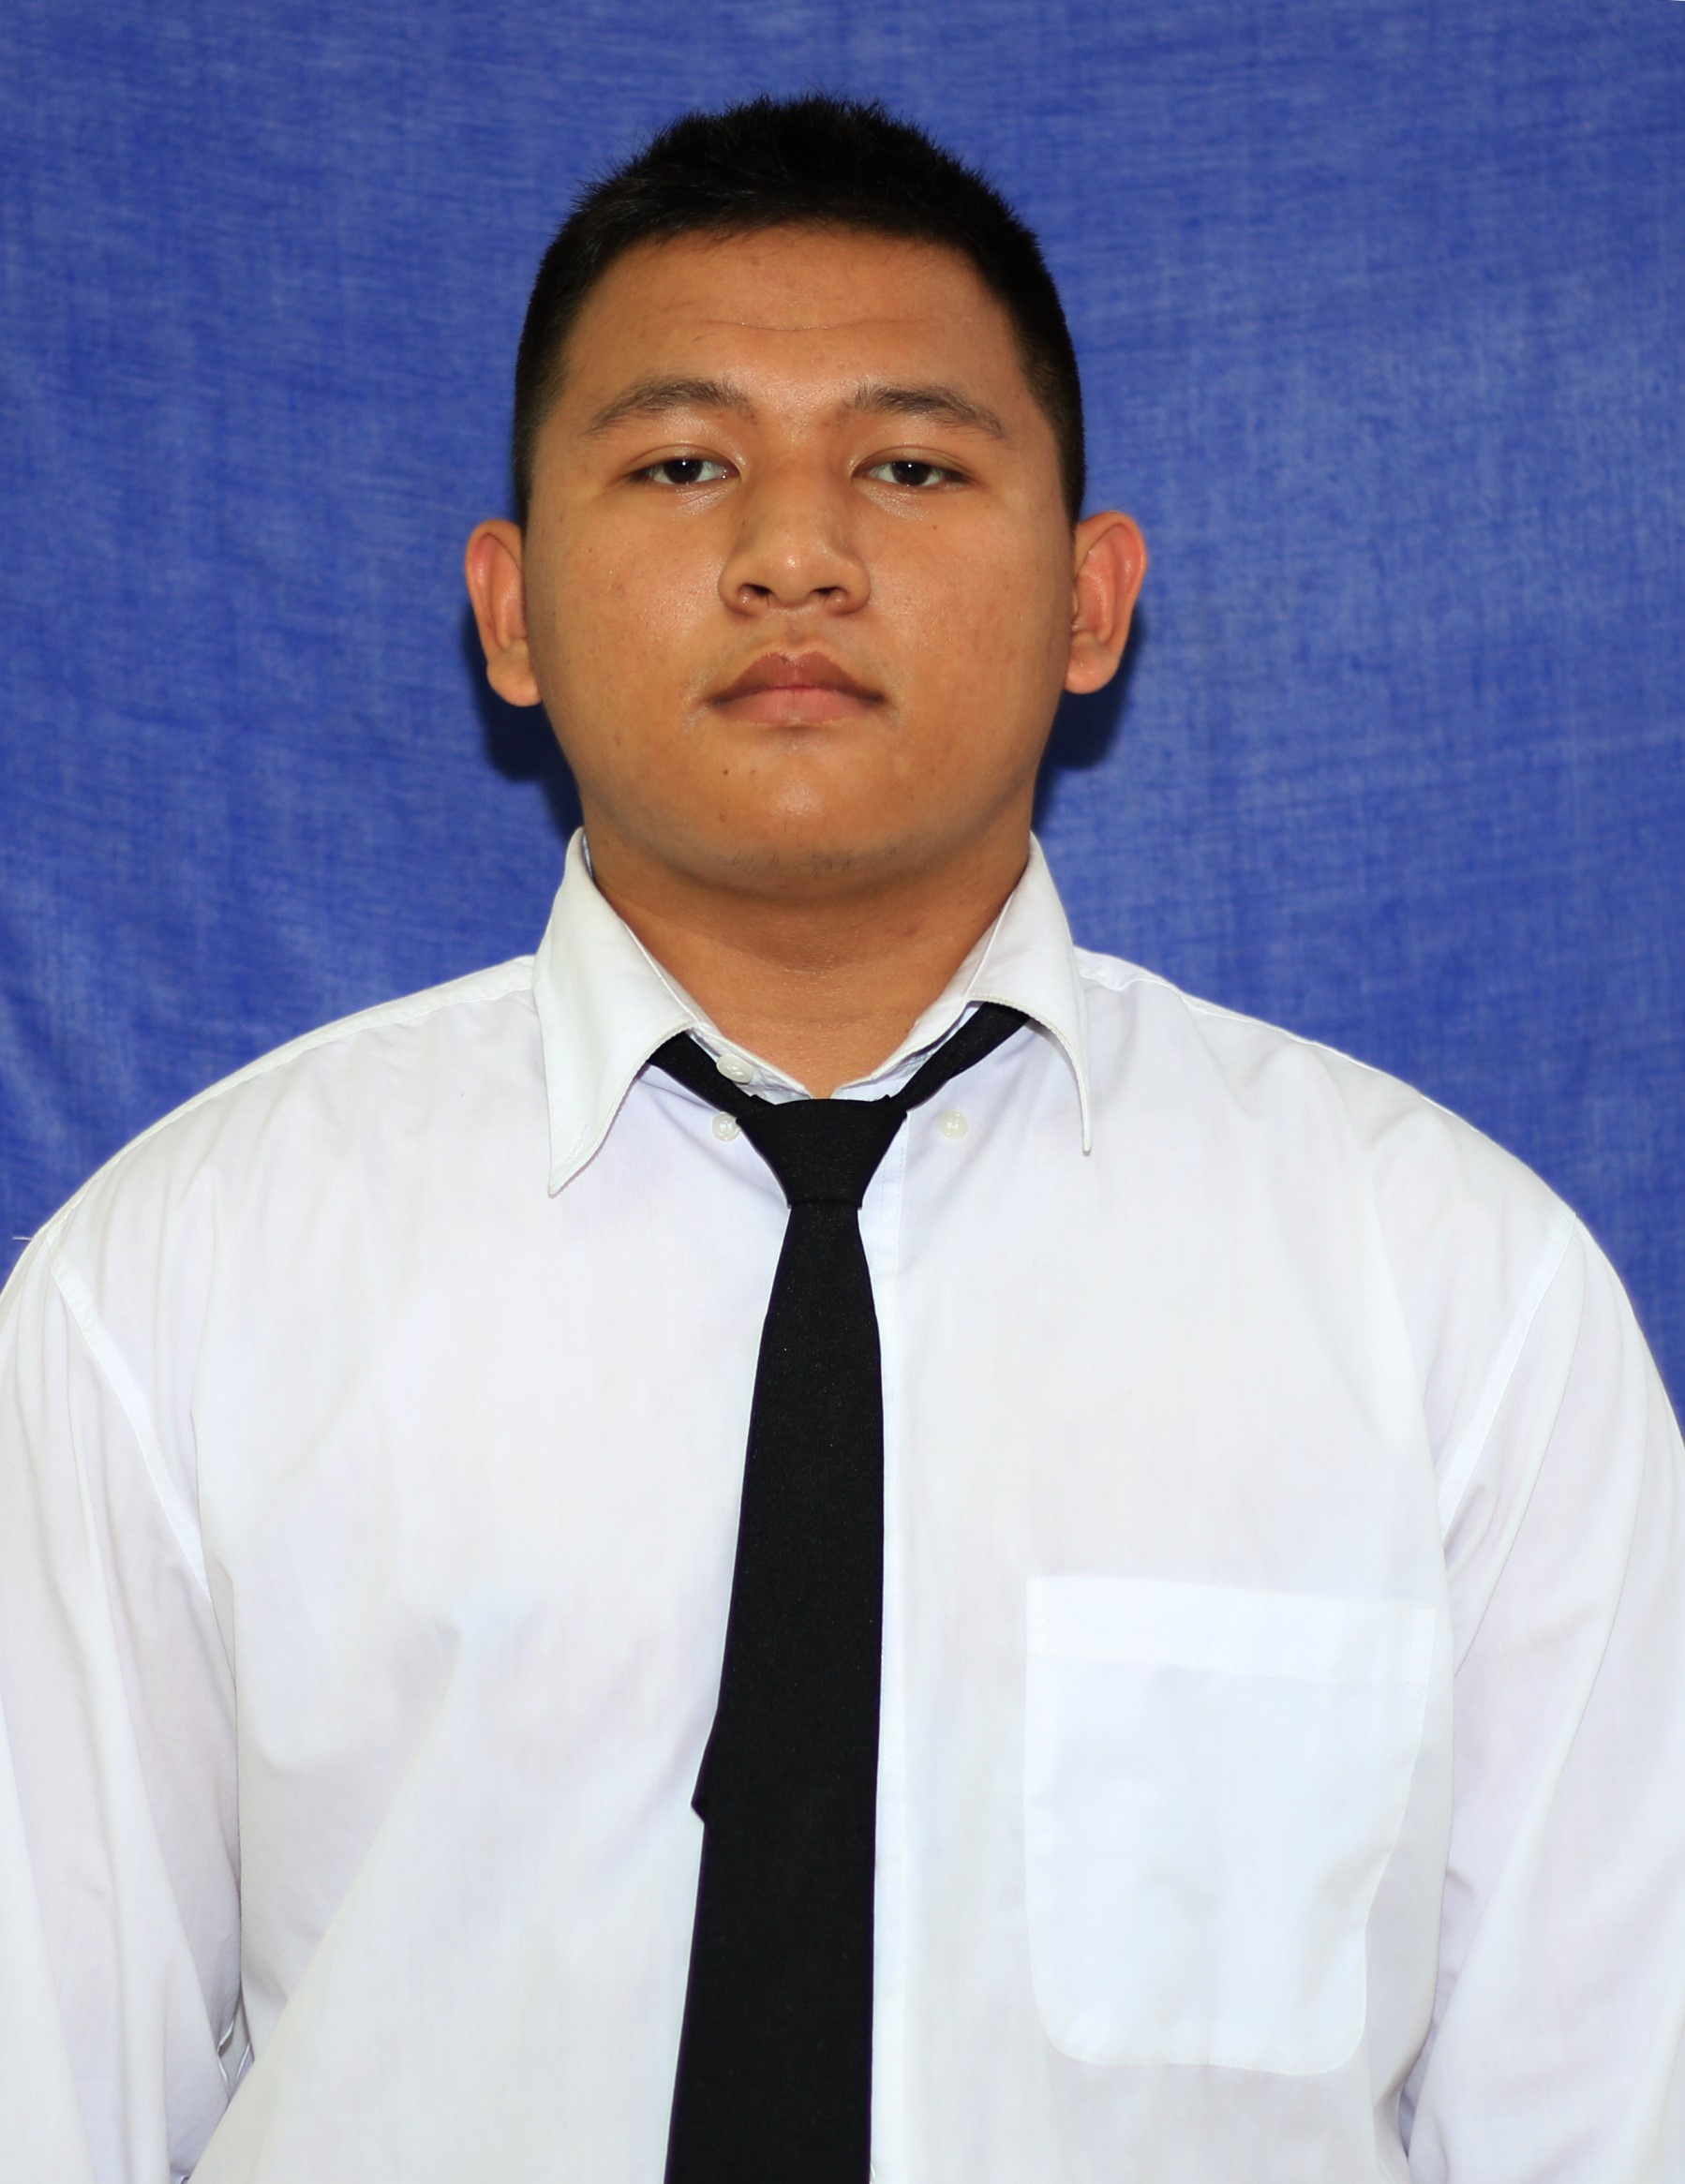
\includegraphics[width=.4\textwidth]{figures/Fotomhs/1144095.jpg}
  \caption{Ini adalah Iqbal Syarif Awaludin}\label{fig:1144095}
\end{figure}
Berikut adalah kegiatan Internship 2 di Prodi D4 Teknik Informatika tertera pada tabel \ref{table:kegiatanharian}
\begin{table}[!ht]
\centering
\begin{tabular}{ |c|c|c|c|c|c|c|c|c|c| }
\hline
No. & Judul Commit & Baris & Kode Commit & Tanggal \\
\hline
1 & Menambah materi macam2 sensor & (\#42) & 2f5ff92660a69b15c4ea4c4c1fd54a4dcdf02f83 & 25/02/2019 \\
\hline
2 & Membuat poster Sistem antrian dan menambah materi Arduino IDE & (\#43) & b9f90a23a64fba1616df40096016e833c9609e78 & 26/02/2019 \\
\hline
3 & Mengedit buku IOT khususnya bagian Software, Mengedit Laporan2019 khususnya rekomendasi kelulusan dan penilaian & (\#2) & ace406d89cdb4a64623650a1f3b4c8aa4e223635 & 27/02/2019 \\
\hline
\end{tabular}
\caption{Tabel Kegiatan Harian}
\label{table:kegiatanharian}
\end{table}
\subsection{28/02/2019}
\begin{enumerate}
  \item Evaluasi mingguan dari jam 9 pagi s/d istirahat.
  \item Koreksi Laporan Proyek 2 Mahasiswa pada format laporan baik itu margin, EYD, dan Typo pada pukul 15.25 s/d 15.40 .
  \item Menambah materi installasi IDE pada Arkom2019 \#44 pada pukul 15.00 s/d 15.25
  https://github.com/BukuInformatika/Arkom2019/commit/e2c587aa9be2382dc0701bda0a4839f6556289ee
  \item Membantu memperbaiki error merge dan conflict pada saat akan pull request milik Daniel S.P. pada pukul 16.40 s/d 17.00.
  \item Merapikan kembali Meja Ibu Noviana pada pukul 17.00.

\end{enumerate}

\subsection{01/03/2019}
\begin{enumerate}
  \item Absen pada pukul 08.57 pagi.
  \item Mengupdate dan memperbaiki penulisan \textbf{chapter1.tex} pada Laporan2019 pada pukul 09.30.
  \item Membantu memperbaiki error merge dan konflik pada saat akan pull request milik Daniel S.P. pada pukul 10.00 s/d selesai.
  \item Mendiskusikan prihal materi tambahan untuk manajemen konflik di git bersama dengan Pak Rolly pada pukul 11.00.
  \item Sosialisasi Internship 2 pukul  14.00 s/d selesai pukul 16.00
  \item Membantu mengabsen peserta sosialisasi Internship 2 selama sosialisasi berlangsung.
  \item Menambahkan materi manajemen konflik yang sudah disetujui oleh Pak Rolly pada pukul 16.05 sampai selesai.
  \par https://github.com/isawaludin/git/commit/6659fa8d574149a084658e88699e7c24531112d0
  \item Merapikan kembali Meja Ibu Noviana pada pukul 17.00.
  \item Pulang pada pukul 17.05 sore.

\end{enumerate}

\subsection{01/03/2019}
\begin{enumerate}
  \item Absen pada pukul 08.57 pagi.
  \item Mengupdate dan memperbaiki penulisan \textbf{chapter1.tex} pada Laporan2019 pada pukul 09.30.
  \item Membantu memperbaiki error merge dan konflik pada saat akan pull request milik Daniel S.P. pada pukul 10.00 s/d selesai.
  \item Mendiskusikan prihal materi tambahan untuk manajemen konflik di git bersama dengan Pak Rolly pada pukul 11.00.
  \item Sosialisasi Internship 2 pukul  14.00 s/d selesai pukul 16.00
  \item Membantu mengabsen peserta sosialisasi Internship 2 selama sosialisasi berlangsung.
  \item Menambahkan materi manajemen konflik yang sudah disetujui oleh Pak Rolly pada pukul 16.05 sampai selesai.
  \par https://github.com/isawaludin/git/commit/6659fa8d574149a084658e88699e7c24531112d0
  \item Merapikan kembali Meja Ibu Noviana pada pukul 17.00.
  \item Pulang pada pukul 17.05 sore.
\end{enumerate}

\subsection{Score Mingguan}
Total score mingguan adalah 15 keterangan seperti pada Tabel \ref{table:scoremingguan}.
\begin{table}[!ht]
\centering
\begin{tabular}{ |c|c|c|c|c|c|c|c|c|c| }
\hline
Kategori & Keterangan Nilai \\
\hline
Dedikasi & 3 \\
\hline
Produktif & 3 \\
\hline
Integritas & 3 \\
\hline
Disiplin & 3 \\
\hline
Loyalitas & 3 \\
\hline
\end{tabular}
\caption{Tabel Score Mingguan}
\label{table:scoremingguan}
\end{table}

\subsection{04/03/2019}
\begin{enumerate}
  \item Masuk pukul 08.55 pagi
  \item Menambah materi manajemen konflik \#12 pukul 09.00 s/d istirahat
  \par https://github.com/BukuInformatika/git/commit/b377a312a6ba75dcbf9046110a43cc8da25ef63d
  \item Masuk setelah istirahat 13.06
  \item Mendiskusikan Repositori baru untuk Internship 2 dan Ta dengan pihak IRC.
  \item Merapihkan kembali meja Bu Noviana pukul 16.55
  \item Pulang pukul 17.00
\end{enumerate}

\subsection{05/03/2019}
\begin{enumerate}
  \item Masuk pukul 08.45 pagi
  \item Mengoreksi Laporan Proyek 1 dan Internship 1 Mahasiswa dari pukul 10.00 s/d istirahat
  \item Masuk setelah istirahat 13.05
  \item Menambah proses install IDE di buku IoT \#9 pukul 15.00
  \par https://github.com/BukuInformatika/IoT/pull/9/commits/e6dae694976bded14b4a6e23baaef0694b01b3bc
  \item Merapihkan kembali meja Bu Noviana pukul 17.00
  \item Pulang pukul 17.00
\end{enumerate} 
\chapter{Harry Syaska Perdana (1144026)}
\section{Laporan Kegiatan Minggu Pertama}
\subsection{Senin, 25 Februari 2019}
\begin{enumerate}
\item \textbf{Dedikasi}
\subitem Git\#8
\item \textbf{Produktif}
\subitem mengikuti kelas pemrograman 3 materi python, kegiatan yang dilakukan menginstall python dan juga anaconda
\item \textbf{Integritas}
\subitem Tidak ada penolakan dalam pull request
\item \textbf{Disiplin}
\subitem Jam Masuk : 08.25 wib
\subitem Jam Keluar : 18.00 wib
\item \textbf{Loyalitas}
\subitem Membantu menata komputer untuk digunakan sebagai sistem antrian
\end{enumerate}

\subsection{Selasa, 26 Februari 2019}
\begin{enumerate}
\item \textbf{Dedikasi}
\subitem Git\#9
\subitem SistemOperasi\#57
\item \textbf{Produktif}
\subitem Membuat tutorial fungsi menambahkan file dan VI editor pada bash
\item \textbf{Integritas}
\subitem Tidak ada penolakan dalam pull request
\item \textbf{Disiplin}
\subitem Jam Masuk : 09.00 wib
\subitem Jam Keluar : 17.00 wib
\item \textbf{Loyalitas}
\subitem Merapihkan kursi di meja pak fachri dan menutup jendela
\end{enumerate}

\subsection{Rabu, 27 Februari 2019}
\begin{enumerate}
\item \textbf{Dedikasi}
\subitem Git\#10
\item \textbf{Produktif}
\subitem Menganalisis dan membuat database perwalian
\subitem menambahkan perintah dasar VI editor pada bash 
\item \textbf{Integritas}
\subitem Tidak ada penolakan dalam pull request
\item \textbf{Disiplin}
\subitem Jam Masuk : 09.00 wib
\subitem Jam Keluar : 17.00 wib
\item \textbf{Loyalitas}
\subitem Merapihkan kursi yang diduduki di meja pak roni habibi
\end{enumerate}

\subsection{Kamis, 28 Februari 2019}
\begin{enumerate}
\item \textbf{Dedikasi}
\subitem SistemOperasi\#58
\item \textbf{Produktif}
\subitem Mengikuti evaluasi yang dilaksanakan diprodi
\subitem Mendiskusikan konten video mingguan
\subitem Melanjutkan menganalisis tentang perwalian 
\item \textbf{Integritas}
\subitem Tidak ada penolakan dalam pull request
\item \textbf{Disiplin}
\subitem Jam Masuk : 08.30 wib
\subitem Jam Keluar : 17.15 wib
\item \textbf{Loyalitas}
\subitem Merapihkan kursi dan meja yang digunakan di meja pak fachri 
\end{enumerate}

\subsection{Jumat, 01 Maret 2019}
\begin{enumerate}
\item \textbf{Dedikasi}
\subitem SistemOperasi\#59
\item \textbf{Produktif}
\subitem Mengikuti sosialisasi Internship 2
\item \textbf{Integritas}
\subitem Tidak ada penolakan dalam pull request
\item \textbf{Disiplin}
\subitem Jam Masuk : 08.50 wib
\subitem Jam Keluar : 17.15 wib
\item \textbf{Loyalitas}
\subitem Membooking ruangan auditorium ke ruang properti untuk sosialisasi internship 2
\end{enumerate}

\subsection{Score Mingguan} 
Tanggal 25 Februari - 1 Maret 2019 Total skor diminggu pertama yaitu \textbf{15}

\begin{table}[h]
\caption{Skor Mingguan}
\centering
\begin{tabular}{|c|c|}
\hline
\textbf{Kategori}&\textbf{Keterangan Nilai}\\
\hline
Dedikasi&03\\
\hline
Produktif&03\\
\hline
Integritas&03\\
\hline
Disiplin&03\\
\hline
Loyalitas&03\\
\hline
\end{tabular}
\label{table : skor mingguan hary}
\end{table}

\subsection{Senin, 04 Maret 2019}
\begin{enumerate}
\item \textbf{Dedikasi}
\subitem SistemOperasi\#60
\item \textbf{Produktif}
\subitem Menambahkan perintah dasar unix di buku sistem operasi
\subitem Briefing dengan IRC mengenai format repositori internship 2 dan TA
\item \textbf{Integritas}
\subitem Tidak ada penolakan dalam pull request
\item \textbf{Disiplin}
\subitem Jam Masuk : 08.55 wib
\subitem Jam Keluar : 17.00 wib
\item \textbf{Loyalitas}
\subitem membelikan makanan untuk prodi 
\end{enumerate}

\subsection{Selasa, 05 Maret 2019}
\begin{enumerate}
\item \textbf{Dedikasi}
\subitem SistemOperasi\#61
\item \textbf{Produktif}
\subitem Menambahkan perintah dasar unix yang sebelumnya di buku sistem operasi
\item \textbf{Integritas}
\subitem Tidak ada penolakan dalam pull request
\item \textbf{Disiplin}
\subitem Jam Masuk : 08.40 wib
\subitem Jam Keluar : 17.00 wib
\item \textbf{Loyalitas}
\subitem memfotocopy dan menjilid buku panduan latex
\subitem membereskan dan merapihkan meja dan kursi prodi
\end{enumerate}

\subsection{Rabu, 06 Maret 2019}
\begin{enumerate}
\item \textbf{Dedikasi}
\subitem Jurnal CNN tentang Automatic Detection of Cerebral Microbleeds from
MR Images via 3D Convolutional Neural Networks
\item \textbf{Produktif}
\subitem membantu mencari jurnal CNN menggunakan MRI dari pak rolly
\item \textbf{Integritas}
\subitem Tidak ada penolakan dalam pull request
\item \textbf{Disiplin}
\subitem Jam Masuk : 08.40 wib
\subitem Jam Keluar : 18.21 wib
\item \textbf{Loyalitas}
\subitem membelikan makanan dan minuman untuk rapat dosen
\end{enumerate}

\subsection{Kamis, 07 Maret 2019}
Tanggal merah

\subsection{Jumat, 08 Maret 2019}
\begin{enumerate}
\item \textbf{Dedikasi}
\subitem git\#16
\item \textbf{Produktif}
\subitem Belajar gitlab mengenai hirarki user 
\item \textbf{Integritas}
\subitem Tidak ada penolakan dalam pull request
\item \textbf{Disiplin}
\subitem Jam Masuk : 09.05 wib
\subitem Jam Keluar : 17.15 wib
\item \textbf{Loyalitas}
\subitem membereskan meja dan kursi yang telah digunakan
\end{enumerate}

\subsection{Score Mingguan} 
Tanggal 04 Maret - 08 Maret 2019 Total skor diminggu pertama yaitu \textbf{13}

\begin{table}[h]
\caption{Skor Mingguan}
\centering
\begin{tabular}{|c|c|}
\hline
\textbf{Kategori}&\textbf{Keterangan Nilai}\\
\hline
Dedikasi&03\\
\hline
Produktif&03\\
\hline
Integritas&03\\
\hline
Disiplin&02\\
\hline
Loyalitas&02\\
\hline
\end{tabular}
\label{table : skor minggu kedua}
\end{table}

\subsection{Senin, 11 Maret 2019}
\begin{enumerate}
\item \textbf{Dedikasi}
\subitem git\#17
\item \textbf{Produktif}
\subitem Berdiskusi tentang github dan gitlab di ruangan kaprodi 
\item \textbf{Integritas}
\subitem Tidak ada penolakan dalam pull request
\item \textbf{Disiplin}
\subitem Jam Masuk : 09.05 wib
\subitem Jam Keluar : 17.15 wib
\item \textbf{Loyalitas}
\subitem memnempelkan grafik data mahasiswa
\subitem merapihkan meja bu noviana
\end{enumerate}

\subsection{Selasa, 12 Maret 2019}
\begin{enumerate}
\item \textbf{Dedikasi}
\subitem -
\item \textbf{Produktif}
\subitem Berdiskusi tentang gitlab di ruangan kaprodi 
\subitem Membuat tutorial menggunakan gitlab di sisi mahasiswa
\item \textbf{Integritas}
\subitem -
\item \textbf{Disiplin}
\subitem Jam Masuk : 08.38 wib
\subitem Jam Keluar : 17.00 wib
\item \textbf{Loyalitas}
\subitem membeli air mineral bareng firman
\end{enumerate}

\subsection{Rabu, 13 Maret 2019}
\begin{enumerate}
\item \textbf{Dedikasi}
\subitem SistemOperasi\#62
\item \textbf{Produktif}
\subitem Mempelajari Gitlab dengan pak harry 
\item \textbf{Integritas}
\subitem Tidak ada penolakan dalam pull request
\item \textbf{Disiplin}
\subitem Jam Masuk : 08.45 wib
\subitem Jam Keluar : 17.00 wib
\item \textbf{Loyalitas}
\subitem membereskan meja pak fachri
\end{enumerate}

\subsection{Kamis, 14 Maret 2019}
\begin{enumerate}
\item \textbf{Dedikasi}
\subitem SistemOperasi\#63
\item \textbf{Produktif}
\subitem Mempelajari dan mempraktekan gitlab dengan anak irc 
\item \textbf{Integritas}
\subitem Tidak ada penolakan dalam pull request
\item \textbf{Disiplin}
\subitem Jam Masuk : 08.48 wib
\subitem Jam Keluar : 17.00 wib
\item \textbf{Loyalitas}
\subitem mecari ruangan untuk sosialisasi proyek 1
\end{enumerate}

\subsection{Jumat, 15 Maret 2019}
\begin{enumerate}
\item \textbf{Dedikasi}
\subitem SistemOperasi\#64
\item \textbf{Produktif}
\subitem Mempraktekan kembali penggunaan gitlab 
\item \textbf{Integritas}
\subitem Tidak ada penolakan dalam pull request
\item \textbf{Disiplin}
\subitem Jam Masuk : 08.48 wib
\subitem Jam Keluar : 17.00 wib
\item \textbf{Loyalitas}
\subitem merapihkan meja pak roni habibi
\end{enumerate}

\subsection{Score Mingguan} 
Tanggal 11 Maret - 15 Maret 2019 Total skor diminggu ketiga yaitu \textbf{12}

\begin{table}[h]
\caption{Skor Mingguan}
\centering
\begin{tabular}{|c|c|}
\hline
\textbf{Kategori}&\textbf{Keterangan Nilai}\\
\hline
Dedikasi&02\\
\hline
Produktif&03\\
\hline
Integritas&02\\
\hline
Disiplin&02\\
\hline
Loyalitas&03\\
\hline
\end{tabular}
\label{table : skor minggu ketiga}
\end{table}

\subsection{Senin, 18 Maret 2019}
\begin{enumerate}
\item \textbf{Dedikasi}
\subitem SistemOperasi\#65
\item \textbf{Produktif}
\subitem Mencari jurnal untuk internship 2 dan TA
\subitem Mempelajari metode yang akan digunakan di TA
\item \textbf{Integritas}
\subitem Tidak ada penolakan dalam pull request
\item \textbf{Disiplin}
\subitem Jam Masuk : 09.11 wib
\subitem Jam Keluar : 17.00 wib
\item \textbf{Loyalitas}
\subitem merapihkan meja pak fachri
\end{enumerate}

\chapter{Daniel Panjaitan (1144085)}
\chapter{Silviana I. Y. Sipahelut (1144112)}
\section{Tabel Kegiatan Senin,25 Februari 2019}
Berikut dibawah ini saya lampirkan daftar kegiatan saya hari ini
\begin{table}[h]
\caption{Tabel Kegiatan}
\centering
\begin{tabular}{|c|c|}
\hline
No&Nama Kegiatan\\
\hline
1&Memperbaiki isi artikel\\
\hline
2&Memperbaiki buku jarkom\\
\hline
\end{tabular}
\label{table:Laporan kegiatan}
\end{table}

\section{Tabel Kegiatan Selasa,26 Februari 2019}
Berikut dibawah ini saya lampirkan daftar kegiatan saya hari ini
\begin{table}[h]
\caption{Tabel Laporan}
\centering
\begin{tabular}{|c|c|}
\hline
No&Nama kegiatan\\
\hline
1&Memperbaiki buku jarkom\\
\hline
2&Memasukan daftar isi dan halaman pada buku jaringan Pa Yusril\\
\hline
\end{tabular}
\label{table:Laporan kegiatan}
\end{table}
\chapter{Dinan Sagara (1144037)}

\section{Senin, 25 Februari 2019}
Kegiatan yang dilakukan pada hari ini
\begin{enumerate}
\item Menyetor Form mengulang Internship 2 dan TA ke BAAK
\item membaca ulang materi Phalcon framework via TutorialsPoint
\item Briefing dengan Pak Rolly mengenai seminar Phalcon
\item Menyusun pertanyaan kuesioner kualitas pelayanan dengan prodi sebanyak 30 pertanyaan
\end{enumerate}

\section{Selasa, 26 Februari 2019}
Kegiatan yang dilakukan pada hari ini
\begin{enumerate}
\item Revisi Laporan Proyek Adik Tingkat
\item Membantu meyusun dan merapikan format buku AJAR (Jaringan Komputer)
\item Mempelajari cara mengubah format file .SVG ke . CDR
\item Menambah materi di Chapter 2 repositori Phalcon.
\subitem https://github.com/BukuInformatika/phalcon/pull/9 dan https://github.com/BukuInformatika/phalcon/pull/10
\end{enumerate}

\section{Rabu, 27 Februari 2019}
Tidak masuk (tanpa adanya alasan)

Link Repositori yang Saya kerjakan di buku Informatika (dan di-fork ke repo Saya) :
\begin{itemize}
\item https://github.com/dsagara/phalcon/commits/master
\end{itemize} 
\chapter{Firman Rasyid Purnama (1144113)}

\section{Senin, 25 Februari 2019}
\begin{itemize}
\item Dedikasi
\subitem Keleketex\#52
\item Produktif
  \subitem Menambahkan penulisan rumus array atau matriks pada buku informatika bagian keleketex chapter 3 materi notifikasi matematis dan merapihkan bab yang memiliki materi perumusan
  \subitem Mengikuti kelas python pada mata kuliah Pak Rolly sebagai pembelajaran tambahan
  \subitem Menyelesaikan tugas membuat sistem antrian mahasiswa untuk di aplikasikan di dalam prodi
  \subitem Briefing dengan Pak Rolly dan Pak Yusril mengenai tugas Buku IoT
\item Integritas
  \subitem Tidak ada penolakan dalam Pull Request
\item Disiplin
  \subitem Jam Masuk : 09.00 wib
  \subitem Jam Pulang :18.00 wib
\item Loyalitas
  \subitem Membantu pak paulus memindahkan komputer admin menerapkan sistem antrian diprodi
  \subitem Merapihkan dan menata kembali tata ruangan komputer admin dengan teman-teman lainnya
\end{itemize}

\section{Selasa, 26 Februari 2019}
\begin{itemize}
\item Dedikasi
  \subitem Keleketex\#56
\item Produktif
  \subitem Menambahkan Tutorial Mengedit file atau dokumen menggunakan editor latex pada buku informatika bagian keleketex chapter 0
  \subitem Memperbaharui Sistem Antrian Mahasiswa
  \subitem Briefing dengan Danil dan Arifmengenai tugas Buku Informatika bagian IoT
\item Integritas
  \subitem Tidak ada penolakan dalam Pull Request
\item Disiplin
  \subitem Jam Masuk : 09.00 wib
  \subitem Jam Pulang :17.15 wib
\item Loyalitas
  \subitem Merapihkan dan menata kembali meja pak roni habibi
\end{itemize}

\section{Rabu, 27 Februari 2019}
\begin{itemize}
\item Dedikasi
  \subitem Keleketex\#58
\item Produktif
  \subitem Datang terlambat karena mengurus nenek yang sakit terlebih dahulu
  \subitem Mengubah isi dan menambahkan materi pada bab 3  dan menambahkan materi perumusan vektor pada bab 4 di buku informatika bagian keleketex.
  \subitem Mempelajari dashboard mahasiswa
\item Integritas
  \subitem Tidak ada penolakan dalam Pull Request
\item Disiplin
  \subitem Jam Masuk : 13.00 wib
  \subitem Jam Pulang :17.00 wib
\item Loyalitas
  \subitem Merapihkan dan menata kembali meja pak roni habibi
\end{itemize}

\section{Kamis, 28 Februari 2019}
\begin{itemize}
\item Dedikasi
  \subitem Keleketex\#60
  \subitem IoT\#5
\item Produktif
  \subitem Mengikuti evaluasi mingguan yang dilaksanakan pak rolly
  \subitem Mendokumentasikan kegiatan evaluasi
  \subitem Mengerjakan tugas Buku IoT dengan menambahkan materi dari jenis-jenis protokol
  \subitem Mendiskusikan konten video mingguan
  \subitem Mengelola sistem antrian admin
\item Integritas
  \subitem Tidak ada penolakan dalam Pull Request
\item Disiplin
  \subitem Jam Masuk : 09.00 wib
  \subitem Jam Pulang :17.15 wib
\item Loyalitas
  \subitem Merapihkan dan menjaga kebersihan meja milik pak roni habibi dan pak cahyo sebelum pulang
\end{itemize}

\section{Jum'at, 01 Maret 2019}
\begin{itemize}
\item Dedikasi
  \subitem Keleketex\#62
\item Produktif
  \subitem Membuat absensi prodi bulan maret
  \subitem Mengikuti Sosialisasi Internship 2
  \subitem Mempelajari penerapan rumus kombinasi pada latex
\item Integritas
  \subitem Tidak ada penolakan dalam Pull Request
\item Disiplin
  \subitem Jam Masuk : 08.50 wib
  \subitem Jam Pulang :17.15 wib
\item Loyalitas
  \subitem Membersihkan kertas sampah yang berserakan dibawah tempat sampah
  \subitem Menghapus papan tulis
  \subitem Membooking ruangan auditorium ke properti untuk sosialisasi internship 2 
\end{itemize}

\subsection{Score Mingguan dari Tanggal 25 Februari - 1 Maret 2019}
Total Score untuk minggu ini adalah 14

\begin{table}[h]
\caption{Score Mingguan}
\centering
\begin{tabular}{|c|c|}
\hline
\textbf{Kategori}&\textbf{Keterangan Nilai}\\
\hline
Dedikasi&03\\
\hline
Produktif&03\\
\hline
Integritas&03\\
\hline
Disiplin&02\\
\hline
Loyalitas&03\\
\hline
\end{tabular}
\label{table:score mingguan}
\end{table}

\section{Senin, 04 Maret 2019}
\begin{itemize}
\item Dedikasi
\subitem Keleketex\#64
\item Produktif
  \subitem Menambahkan penulisan tata letak pada sebuah rumus
  \subitem Mempelajari arduino
  \subitem Mencari jurnal mengenai sistem lock door menggunakan arduino dan RFID 
  \subitem Briefing dengan pihak IRC mengenai format repositori Internship 2 dan TA
\item Integritas
  \subitem Tidak ada penolakan dalam Pull Request
\item Disiplin
  \subitem Jam Masuk : 08.54 wib
  \subitem Jam Pulang :17.00 wib
\item Loyalitas
  \subitem Membelikan air mineral vit 1 dus untuk prodi
  \subitem Menata air mineral vit di depan admin
\end{itemize}

\section{Selasa, 05 Maret 2019}
\begin{itemize}
\item Dedikasi
\subitem git\#13
\subitem git\#14
\item Produktif
  \subitem Membuat tutorial cara membaca pull request pada buku git
  \subitem Membuat Standar untuk melakukan approve pada github
\item Integritas
  \subitem Tidak ada penolakan dalam Pull Request
\item Disiplin
  \subitem Jam Masuk : 08.56 wib
  \subitem Jam Pulang :17.00 wib
\item Loyalitas
  \subitem Menfotocopy dan menjilid buku panduan git 
  \subitem Menghapus papan tulis
  \subitem Membereskan dan merapihkan meja-meja prodi
  \subitem Membersihkan dispenser prodi 
\end{itemize}







\appendix
\chapter{Form Penilaian Jurnal}

gambar \ref{form1} dan \ref{form2} merupakan contoh bagaimana reviewer menilai jurnal kita. 
\begin{figure}[ht]
      \centerline{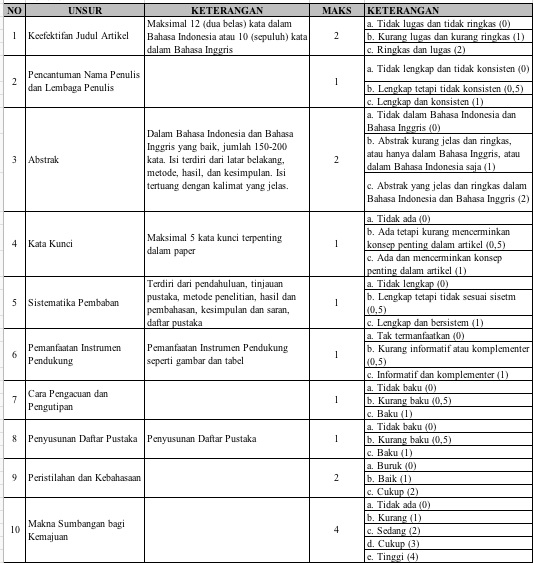
\includegraphics[width=1\textwidth]
      {figures/form1}}
      \caption{Form nilai bagian 1.}
      \label{form1}
      \end{figure}

	\begin{figure}[ht]
	      \centerline{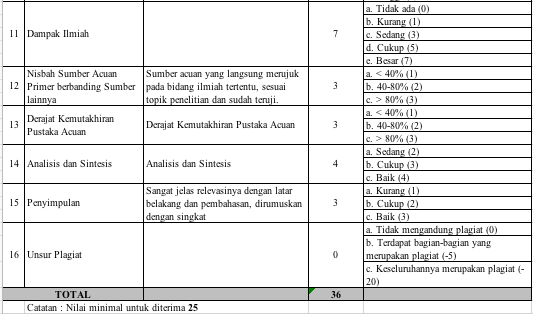
\includegraphics[width=1\textwidth]
	      {figures/form2}}
	      \caption{form nilai bagian 2.}
	      \label{form2}
	      \end{figure}

\chapter{FAQ}

M : Kalo Intership II atau TA harus buat aplikasi ?
D : Ga harus buat aplikasi tapi harus ngoding

M : Pa saya bingung mau ngapain, saya juga bingung mau presentasi apa?
D : Makanya baca de, buka jurnal topik `ganteng' nah kamu baca dulu sehari 5 kali ya, 4 hari udah 20 tuh. Bingung itu tanda kurang wawasan alias kurang baca.

M : Pa saya sudah cari jurnal terindeks scopus tapi ga nemu.
D : Kamu punya mata de? coba dicolok dulu. Kamu udah lakuin apa aja? tolong di list laporkan ke grup Tingkat Akhir. Tinggal buka google scholar klik dari tahun 2014, cek nama jurnalnya di scimagojr.com beres.

M : Pa saya belum dapat tempat intership, jadi ga tau mau presentasi apa?
D : kamu kok ga nyambung, yang dipresentasikan itu yang kamu baca bukan yang akan kamu lakukan.

M : Pa ini jurnal harus yang terindex scopus ga bisa yang lain ?
D : Index scopus menandakan artikel tersebut dalam standar semantik yang mudah dipahami dan dibaca serta bukan artikel asal jadi. Jika diluar scopus biasanya lebih sukar untuk dibaca dan dipahami karena tidak adanya proses review yang baik dan benar terhadap artikel.

M : Pa saya tidak mengerti
D : Coba lihat standar alasan

M : Pa saya bingung
D : Coba lihat standar alasan

M : Pa saya sibuk
D : Mbahmu....

M : Pa saya ganteng
D : Ndasmu....

M : Pa saya kece
D : wes karepmu lah....


Biasanya anda memiliki alasan tertentu jika menghadapi kendala saat proses bimbingan, disini saya akan melakukan standar alasan agar persepsi yang diterima sama dan tidak salah kaprah. Penggunaan kata alasan tersebut antara lain :

1. Tidak Mengerti : anda boleh menggunakan alasan ini jika anda sudah melakukan tahapan membaca dan meresumekan 15 jurnal. Sudah mencoba dan mempraktekkan teorinya dengan mencari di youtube dan google minimal 6 jam sehari selama 3 hari berturut-turut.

2. Bingung : anda boleh mengatakan alasan bingung setelah maksimal dalam berusaha menyelesaikan tugas bimbingan dari dosen(sudah dilakukan semua). Anda belum bisa mengatakan alasan bingung jika anda masih belum menyelesaikan tugas bimbingan dan poin nomor 1 diatas. Setelah anda menyelesaikan tugas bimbingan secara maksimal dan tahap 1 poin diatas, tapi anda masih tetap bingung maka anda boleh memakai alasan ini.

\addcontentsline{toc}{chapter}{Bibliography}

\bibliography{references}
\bibliographystyle{plain}

\end{document}

